\documentclass[12pt,a4paper]{article}

\usepackage[T1]{fontenc} 
\usepackage[utf8]{inputenc}
\usepackage{placeins}
\usepackage[a4paper]{geometry}
\geometry{hscale=0.85,vscale=0.85,centering}
\usepackage{lmodern}
\usepackage{framed}
\usepackage[framed]{ntheorem}
\usepackage{xcolor}
\usepackage{graphicx}
\usepackage{tikz}
\usepackage{subfigure}
\usepackage{wrapfig}
\graphicspath{ {./img/} }
\usepackage{amssymb}
\usepackage{amsmath}
\usepackage{amsfonts}
\usepackage{dsfont}
\usepackage{listings}
\usepackage{titlesec}
\usepackage{pgfplots}
\pgfplotsset{compat=1.12}
\usepackage{url}
\usepackage{hyperref}
\hypersetup{					% setup the hyperref-package options
	breaklinks=true,			% 	- allow line break inside links		%
	colorlinks,
	citecolor=black,
	filecolor=black,
	linkcolor=black,
	urlcolor=black
}

\usepackage[francais]{babel}


\titleformat{\section}
{\centering \Large \normalfont \scshape}{\thesection}{1em}{}
\titleformat{\subsection}
{ \large \scshape}{\thesubsection}{1em}{}
\titleformat{\subsubsection}
{ \normalsize \scshape}{\thesubsubsection}{1em}{}
\numberwithin{equation}{section}


\newcommand{\elevation}{\texttt{Elevation}}
\newcommand{\aspect}{\texttt{Aspect}}
\newcommand{\slope}{\texttt{Slope}}
\newcommand{\hhydro}{\texttt{Horizontal\_Distance\_To\_Hydrology}}
\newcommand{\vhydro}{\texttt{Vertical\_Distance\_To\_Hydrology}}
\newcommand{\roadways}{\texttt{Distance\_To\_Roadways}}
\newcommand{\hilshadeM}{\texttt{Hillshade\_9am}}
\newcommand{\hilshadeN}{\texttt{Hillshade\_Noon}}
\newcommand{\hilshadeA}{\texttt{Hillshade\_3pm}}
\newcommand{\fire}{\texttt{Distance\_To\_Fire\_Points}}
\newcommand{\wilderness}{\texttt{Wilderness\_Area}}
\newcommand{\soil}{\texttt{Soil\_Type}}
\newcommand{\cover}{\texttt{Cover\_Type}}

\title{\scshape \huge Forest Cover Type Prediction}
\author{\textbf{Kevin Zagalo} \\  \url{kevin.zagalo@etu.upmc.fr}  \and \textbf{Ismail Benkirane} \\ \url{ismail.benkirane@etu.upmc.fr}}
\date{}

\begin{document}
	
	\maketitle
	
	{\small Projet pour le cours \textit{Apprentissage Statistique} du LIP6 \footnote[0]{Laboratoire d'Informatique de Paris 6 :: \url{https://www.lip6.fr}}, Sorbonne Université} \hfill Janvier 2019
	
	\hrulefill
	
	\begin{abstract}
		Ce projet a pour but de proposer et tester des modèles pour l'étude de la base de données  \textit{Covertype} \footnote{\url{https://archive.ics.uci.edu/ml/datasets/Covertype}}. Il s'agit d'un problème de classification multi-classe avec 7 classes, 581\,012 instances et 54 attributs sans données manquantes.\\
		
		\begin{flushleft}
			\begin{tabular}{l l p{5.2cm}}
				Nom & Unité & Description \\
				\hline
				\elevation & mètres & Altitude \\ 
				\aspect & degrés & Orientation \\ 
				\slope & degrés & Pente \\
				\hhydro & mètres & Distance horizontale au point d’eau le plus proche\\
				\vhydro & mètres & Distance verticale au point d’eau le plus proche \\
				\roadways & mètres & Distance horizontale à la route la plus proche \\
				\fire & mètres & Distance horizontale au départ de feu le plus proche\\
				\hilshadeM & entier entre 0 et 255 & Ombrage à 9h au solstice d’été \\
				\hilshadeN & entier entre 0 et 255 & Ombrage à 12h au solstice d'été\\
				\hilshadeA & entier entre 0 et 255 &  Ombrage à 15h au solstice d'été \\
				\wilderness & 4 colonnes binaires & Wilderness area designation \\
				\soil & 40 colonnes binaires & Type de sol\\
				\cover & entier entre 1 et 7 & Classe\\
			\end{tabular}
		\end{flushleft}
	\end{abstract}
	
	\tableofcontents
	
	\newpage
	
	\section{Analyse préliminaire et pré-traitement des données}
	
	On choisit d'utiliser la bibliothèque \verb!pandas! pour charger les données, surtout pour l'analyse préliminaire. \verb!pandas! fournit une panoplie de fonctions pour visualiser les données. \verb!groupby!, \verb!boxplot! et \verb!hist! nous seront forts utiles pour choisir les données que nous exploiterons. Le \textit{notebook} contenant le code joint au rapport nécessite aussi les bibliothèques \verb!matplotlib!, \verb!numpy!, \verb!sklearn! et \verb!plotly!.\\
	
	Avant toute modification des données et/ou élaboration de méthodes, nous tenterons de mieux comprendre les données pour éventuellement les modifier, c'est-à-dire :\\
	
	\begin{itemize}
		\item exhiber des corrélations
		\item supprimer des données inutiles
		\item ajouter des données qui seraient plus pertinentes
		\item modifier la façon de "qualifier" les données qualitatives
	\end{itemize}
	
	\medskip
	
	Tout d'abord on constate sur la figure \ref{fig:datahist} que les données sont inégalement réparties selon les classes. Cela peut vouloir dire plusieurs choses : soit nos données sont mal échantillonnées, soit les types \verb!1! et \verb!2! sont effectivement largement plus répandues.\\
	
	\begin{wrapfigure}{r}{0.65\textwidth}
		\centering
		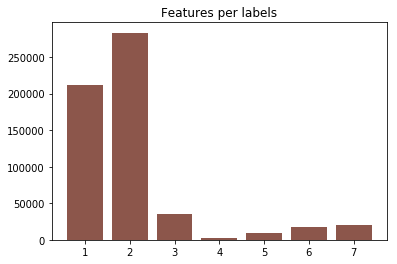
\includegraphics[width=.7\linewidth]{img/data_hist}
		\caption{Histogramme des données par types de forêts}
		\label{fig:datahist}
	\end{wrapfigure}
	
	C'est quelque chose dont nous n'avons pas la maitrise, une discussion avec un expert sur le sujet serait préférable. On prendra donc cela en compte dans nos méthodes.\\
	
	La suite consistera globalement à faire la même chose sur le reste des données grâce aux méthodes de la bibliothèque \verb!pandas!.\\
	
	On observe dans la figure \ref{fig:boxplots} l'importance des attributs \elevation, \slope \ et \  \roadways. 
	
	\begin{figure}[h]
		\centering
		\subfigure[\slope]{
			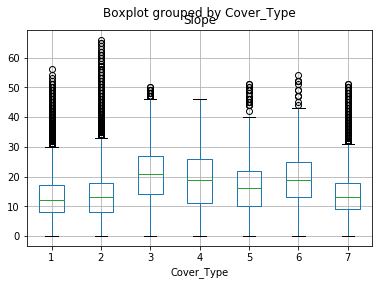
\includegraphics[width=0.3\linewidth]{img/slope_boxplot}
		}
		\hfill
		\subfigure[\roadways]{
			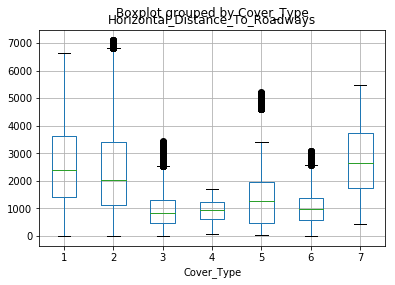
\includegraphics[width=0.3\linewidth]{img/roadways_boxplot}
		}
		\hfill
		\subfigure[\elevation]{
			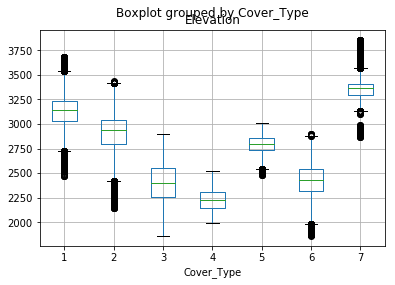
\includegraphics[width=0.3\linewidth]{img/elevation_boxplot}
		}
		\caption{Boxplot des données numériques}
		\label{fig:boxplots}
	\end{figure}
	
	La première partie consistera donc à voir si on peut réduire le nombre de paramètres, la deuxième à modifier les données pour une meilleure analyse, et enfin mettre les données de train, de validation et de test. On trouve déjà quelques idées dans \cite{B-D}.
	
	\subsection{Réduction des paramètres}
	
	Nous le ferons en deux parties : une première fois pour les variables qualitative et la seconde pour les valeurs numériques. On préfèrera garder dans le DataFrame \verb!df_covtype! des entiers plutôt que des vecteurs binaires, quitte à les y remettre dans les données de train et de test ensuite. Cela facilitera grandement l'analyse préliminaire.\\
	
	L'attribut \wilderness n'apporte pas beaucoup d'information, mais elle permet de distinguer la classe 4, qui a du mal a être identifiée par les méthodes testées. En effet, les forêts de classe 4 ne sont que dans 'Cache la poudre'. Nous allons donc garder l'attribut comme un 4-vecteur binaire : 
	
	- 1 : Rawah \ \ \ \ - 2 : Neota  \ \ \ \ - 3: Comanche Peak\ \ \ \ - 4 : Cache la Poudre  
	
	\begin{figure}[h]
		\centering
		\hfill
		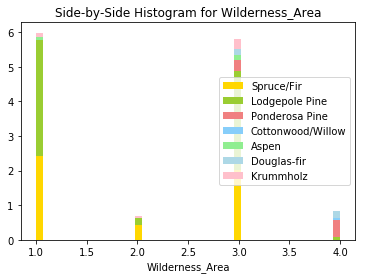
\includegraphics[width=0.35\linewidth]{img/wilderness_hist}
		\hfill
		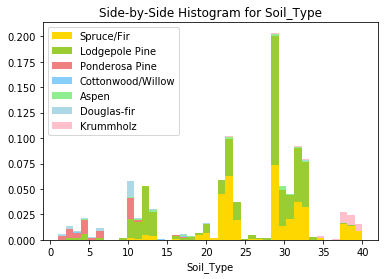
\includegraphics[width=0.35\linewidth]{img/soil_hist}
		\hfill
		\label{fig:wildernesssoilhist}
		\caption{Histogrammes pour \wilderness et \soil}
	\end{figure}
	
	Pour réduire presque de moitié les paramètres de \soil, nous considérerons uniquement les familles de sols, et le fait qu'ils soient rocheux, friable ou autre, pour atteindre le nombre de 24 paramètres. On trouve ces informations dans le fichier \textit{covtype.info} fourni avec les données.\\
	
	-  1 to 40 : based on the USFS Ecological Landtype Units for this study area\\
	
	Nous aurons plutôt deux vecteurs binaires \texttt{soil\_family} et \texttt{soil\_group}, respectivement de taille 3 et 21 qui remplaceront la variable \soil. On remarquera que le deuxième permet entre autres de mieux classer la classe 7, puisqu'elle n'est présente que dans les forêts rocheuses.
	
	\begin{figure}[h]
		\centering
		\hfill
		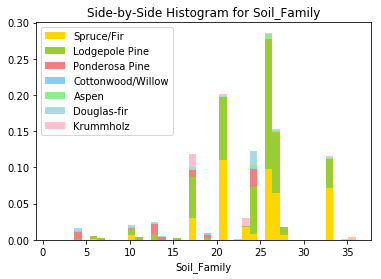
\includegraphics[width=0.35\linewidth]{img/soil_family}
		\hfill
		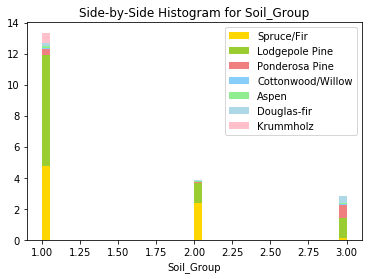
\includegraphics[width=0.35\linewidth]{img/soil_group}
		\hfill
		\label{fig:soilhist}
		\caption{Histogrammes pour \texttt{Soil\_Family} et \texttt{Soil\_Group}}
	\end{figure}
	
	\pagebreak
	
	\subsection{Transformation des données}
	On commence par chercher des corrélations entre les données :
	
	\begin{figure}[h]
		\centering
		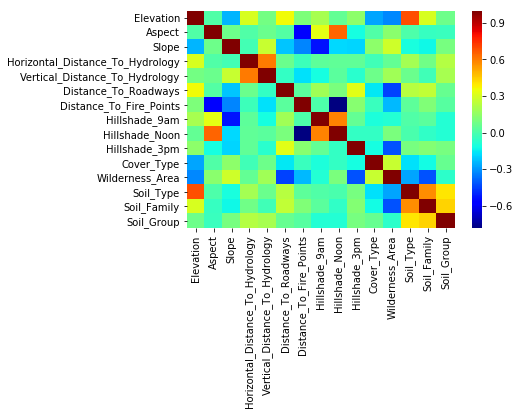
\includegraphics[width=.48\linewidth]{img/corr_matrix}
		\hfill
		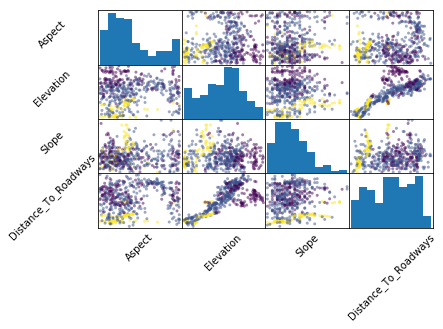
\includegraphics[width=.5\linewidth]{img/scatter_matrix}.
		\caption{Matrices de corrélations}
	\end{figure}
	
	On voit ici plusieurs choses :
	
	\begin{itemize}
		\item Plus la pente est grande, plus l'ombre a de la variance
		\item L'élévation est grandi linéairement en fonction de la distance aux routes
		\item L'azimuth et l'ombrage forment des sigmoid\\
	\end{itemize}
	
	\begin{wrapfigure}{r}{0.5\textwidth}
		\centering
		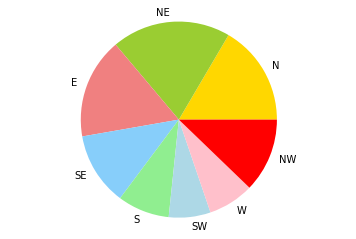
\includegraphics[width=.9\linewidth]{img/aspect}
		\caption{Répartition de \aspect }
		\label{Aspect}
	\end{wrapfigure}
	
	On remplacera \aspect \ par $$\verb!Aspect_Group! = (N,NW,W,SW,S,SE,E,NE)$$ ce qui permet de faire un apprentissage catégoriel plutôt que numérique.\\
	
	On constate sur la figure \ref{Aspect} que la plupart des forêts sont orientées vers le nord-est, et donc il est logique de trouver que l'ombrage à 3 heures de l'après midi soit plus important que les deux autres. On voit que la distribution de \hilshadeA \ ressemble à une gaussienne, ce qui est exploitable. 
	
	\begin{figure}[h]
		\centering
		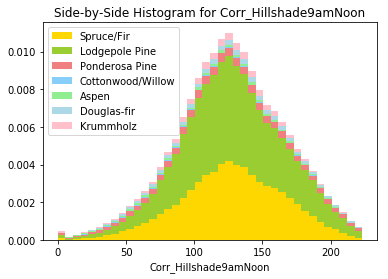
\includegraphics[width=.3\linewidth]{img/corr_hillshade}
		\hfill
		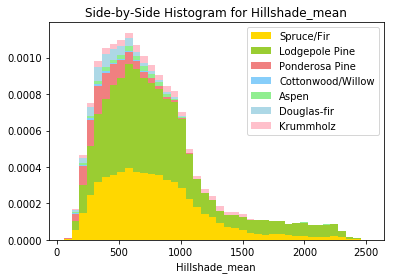
\includegraphics[width=.3\linewidth]{img/hillshade_mean}
		\hfill
		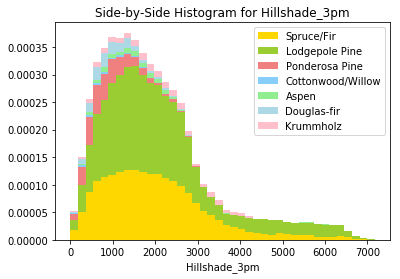
\includegraphics[width=.3\linewidth]{img/hillshade3}
		\caption{Répartitions de \texttt{Corr\_Hillshade9amNoon}, \texttt{Hillshade\_mean} et \hilshadeA}
	\end{figure}
	
	On gardera donc \hilshadeA \ et deux nouveaux attributs $\texttt{Corr\_Hillshade9amNoon} = \hilshadeM \times \hilshadeN /255$ et $$\texttt{Hillshade\_mean} = \frac{\hilshadeM + \hilshadeN+ \hilshadeA}{3}$$
	
	
	L'idée vient du fait qu'en faisant cela, nous nous retrouvons avec une quantité proportionnelle à des distances comme l' \elevation \ ou des polynômes des quantités comme \hilshadeA.\\
	
	\begin{figure}[h]
		\centering
		\hfill
		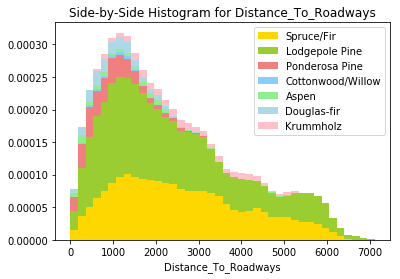
\includegraphics[width=.48\linewidth]{img/roadways_hist}
		\hfill
		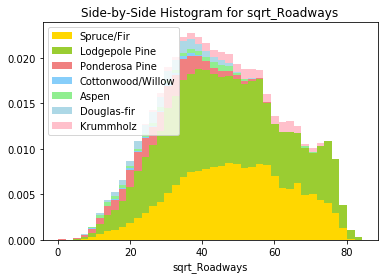
\includegraphics[width=.48\linewidth]{img/sqrt_roadways_hist}
		\hfill
		\caption{Répartitions de \roadways et \texttt{sqrt\_Roadways}}
	\end{figure}
	
	Ensuite, nous voyons sur la figure que la distribution de l'attribut \roadways \ ressemble à une $\chi^2$. Si on en prend la racine carrée on se retrouve donc avec une distribution proche d'une gaussienne. On fera la même chose pour \fire . Pour la distance à l'eau nous résumerons les deux paramètres à la distance euclidienne à l'eau, c'est-à-dire $$ \sqrt{\vhydro^2 + \hhydro^2}$$
	
	\begin{figure}[h]
		\centering
		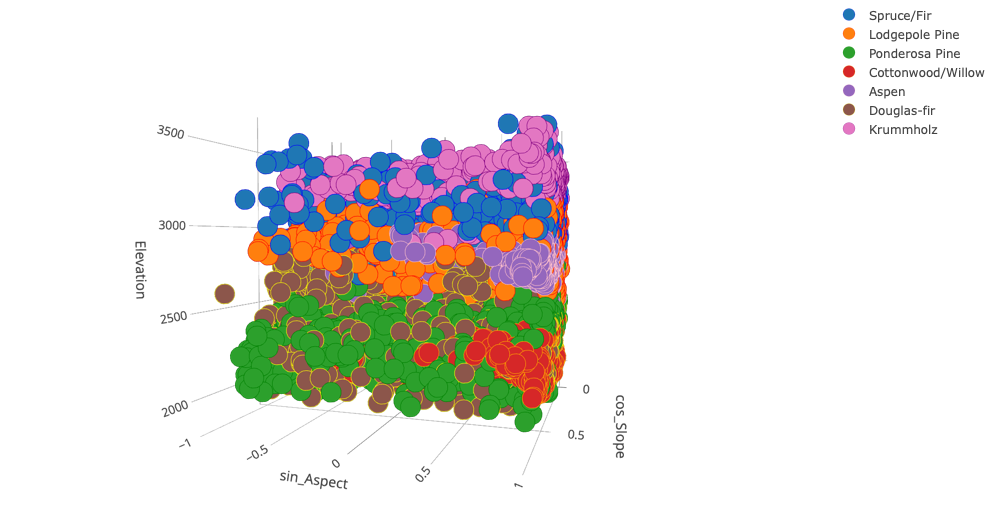
\includegraphics[width=.8\linewidth]{img/sin_aspect}
		\caption{Grapique de \texttt{cos\_Slope}, \texttt{sin\_Aspect} et \elevation}
	\end{figure}
	
	Enfin, nous prendrons les cosinus de nos données quantifiées en degrés et degrés azimuth. Nous aurons donc deux nouveaux attributs \texttt{cos\_Slope} et \texttt{sin\_Aspect} qui sont respectivement le cosinus de la pente des forêts et le sinus de l'orientation par rapport au nord. \\
	
	Une dernière étape consistera à normaliser les colonnes de nos données car elles n'ont pas du tout les mêmes échelles. (voir le code)
	
	\section{Test des méthodes}
	Avant de commencer, nous savons que pour chaque méthode, nous utiliserons l'hyperparamètre \texttt{class\_weights} dès que possible pour pouvoir compenser l'écrasante majorité des classes 1 et 2.\\
	
	Nous étudierons les modèles suivant : 
	
	\begin{itemize}
		\item Logistic Regression
		\item Random Forest
		\item Quadratic Discriminant Analysis
	\end{itemize}
	
	\subsection{Logistic Regression}
	
	On cherche d'abord du côté de la régression logistique multinomiale. Comme elle est sensible aux trop grandes variances, on décide d'utiliser un paramètre de régularisation grâce à la pénalité \textit{elastic net}. La loi a posteriori sachant que les données sont $(\textbf{x},\textbf{y}) = (\textbf{x}^{(i)},\textbf{y}^{(i)})_{i=1}^N$ est une loi multinomiale *(softmax)* 
	$$\Pr (\widehat{y}=k \vert \textbf{w};\textbf{x}) = \frac{\exp(w_{0,k} + \textbf{w}_k .\textbf{x})}{\sum_{j=1}^7 \exp(w_0 + \textbf{w}_j . \textbf{x})} $$ 
	
	et sa fonction de coùt est donc donnée par la log-vraisemblance 
	
	$$- \left[\frac{1}{N} \sum_{i=1}^{N} \left( \sum_{j=1}^7 y^{(i)}_j (w_{0,j} + \textbf{w}_j.\textbf{x}^{(i)}) - \log \sum_{j=1}^7 e^{w_{0,j} + \textbf{w}_j . \textbf{x}^{(i)}} \right) \right] + \lambda \left[ \frac{1 - \alpha}{2} \sum_{j=1}^7 \vert \vert \textbf{w}_j \vert \vert^2 + \alpha \sum_{j=1}^7 \vert \vert \textbf{w}_j \vert \vert \right]$$
	
	où $N$ est le nombre d'observations. Le second terme de l'équation représente le terme de régularisation \textit{elastic net}. Dans la pénalité \textit{elastic net}, $\alpha$ varie de 0 à 1. Quand $\alpha=0$, on a une régularisation L2, quand $\alpha=1$, on a une régularisation L1 ("Lasso"). Quelques test montrent qu'il n'est pas nécessaire de faire varier alpha. Nous nous contenterons donc d'une régularisation L2. Des test préalables montrent que le terme de régularisation est de l'ordre de $10^{-3}$.\\
	
	\begin{wrapfigure}{r}{.5\textwidth}
		\centering
		\begin{tabular}{r cccc}
			& precision & recall &f1-score &  support  \\
			1    &   0.59   &    0.41  &    0.48  &   63498 \\
			2    &   0.65   &   0.60    &  0.62   &  85198 \\
			3    &   0.48   &   0.69   &   0.57  &    10581 \\
			4    &   0.16   &   0.92   &   0.27   &   822 \\
			5    &   0.07   &   0.34    &  0.12     &  2850\\
			6    &   0.25   &   0.19  &    0.21 &     5229\\
			7    &   0.34   & 0.80     & 0.48     & 6126\\
			avg    &    0.58   &   0.53  &    0.54  &  174304	\\
		\end{tabular}
		\caption{Logistic Regression sur les données modifiées avec PCA}
		\label{log pca}
	\end{wrapfigure}
	
	Premièrement, la régression logistique multinomiale ne converge pas sur les données brutes. Sur les données modifiées nous arrivons à une accuracy de \textbf{63.8\%} mais avec un très mauvais rappel pour la plupart des classes. \\
	
	On tente de le résoudre avec un PCA et cela fonctionne plutôt dans l'ensemble : On arrive à un score de \textbf{52,7\%} mais avec un rappel et une precision beaucoup plus équilibrés, comme on le voit dans la figure \ref{log pca}. En fait il est difficile de faire mieux : tous les autres test montrent que les classes 4 et 5 ont  du mal à être détectées. Sans doute faut-il agrandir la taille des features pour pouvoir mieux identifier ces classes.
	
	\subsection{Random Forest}
	Tout d'abord on trie nos attributs grâces aux Forêts Aléatoires. Les données modifiées mettent en avant les attributs 
	
	\begin{figure}[h]
		\centering
		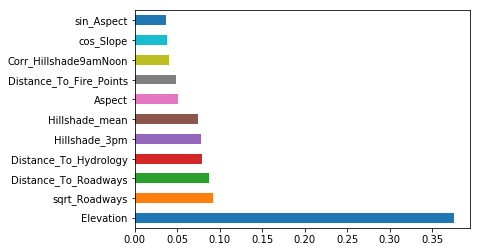
\includegraphics[width=1\linewidth]{img/importance.png}
		\caption{ExtraTreesClassifier sur les données modifiées avec PCA}
	\end{figure}
	
	On fait varier les paramètres de notre premier modèle sur les données brutes. On commence par les paramètres \texttt{n\_estimators}, qui est le nombre d'arbres, et \texttt{max\_depth} qui la profondeur des arbres utilisés dans le modèle. On constate par différents test \footnote{cf. le notebook joint au rapport} qu'aller au delà de 15 et 50 respectivement ne change pas grand chose.\\
	
	\begin{figure}[h]
		\centering
		\subfigure[Learning Curve sans PCA]{
			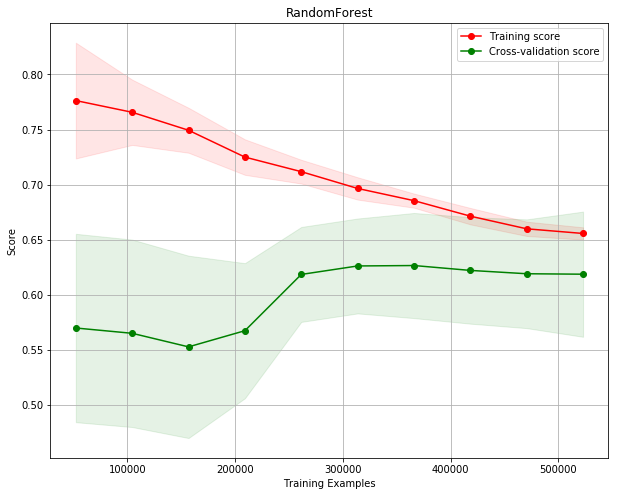
\includegraphics[width=.48\linewidth]{img/rf_sans_pca.png}
		}
		\hfill
		\subfigure[Learning Curve avec PCA]{
			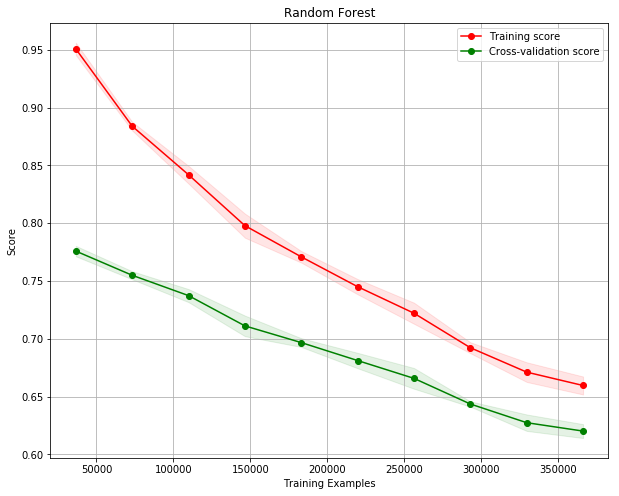
\includegraphics[width=.48\linewidth]{img/rfc_with_PCA.png}
		}
	\end{figure}
	
	\begin{figure}[h]
		
		\subfigure[Rapport de classification sans PCA]{
			\begin{tabular}{r cccc}
				& precision & recall &f1-score &  support  \\
				1    &   0.72   &    0.40  &    0.51  &   63498 \\
				2    &   0.65   &   0.79    &  0.71   &  85198 \\
				3    &   0.61   &   0.86   &   0.72  &    10581 \\
				4    &   0.40   &   0.87    &   0.55    &   822 \\
				5    &   0.24   &   0.11    &  0.15     &  2850\\
				6    &   0.22   &   0.34  &    0.27 &     5229\\
				7    &   0.56   & 0.83     & 0.67     & 6126\\
				avg   &    0.65   &   0.63  &    0.62  &  174304	\\
			\end{tabular}
		}	
		\hfill
		\subfigure[Rapport de classification avec PCA]{
			\begin{tabular}{r cccc}
				& precision & recall &f1-score &  support  \\
				1    &   0.89   &    0.57  &    0.69  &   63498 \\
				2    &   0.82   &   0.61    &  0.70   &  85198 \\
				3    &   0.82   &   0.57   &   0.67  &    10581 \\
				4    &   0.57   &   0.86    &   0.69    &   822 \\
				5    &   0.07   &   0.87    &  0.12     &  2850\\
				6    &   0.31   &   0.89  &    0.46 &     5229\\
				7    &   0.62   & 0.92     & 0.74     & 6126\\
				avg    &    0.81   &   0.62  &    0.68  &  174304	\\
			\end{tabular}
		}	
		\caption{Random Forest sur les données modifiées avec PCA}
	\end{figure}
	
	Finalement, on obtient un score de \textbf{61.7\%} sans le PCA, et \textbf{61.5\%} avec. On préfèrera garder la méthode avec PCA tout de même.
	
	\pagebreak
	
	\bibliographystyle{alphadin}
	\bibliography{covtype}
	
\end{document}